% Use the content.tex file to enter your content.

\documentclass[sigconf, nonacm, screen=True, review=False, anonymous=False, authordraft=False]{acmart}

%%% START ADDITIONAL PACKAGES AND COMMANDS %%%
\renewcommand{\sectionautorefname}{Section}
\renewcommand{\subsectionautorefname}{Section}
\renewcommand{\subsubsectionautorefname}{Section}

\usepackage[yyyymmdd]{datetime}
\renewcommand{\dateseparator}{--}

% \usepackage{enumitem}
\usepackage{tabularx}
\usepackage{dcolumn} %Aligning numbers by decimal points in table columns
\newcolumntype{d}[1]{D{.}{.}{#1}}

\usepackage{subcaption}
\usepackage{tikz}
\usetikzlibrary{arrows.meta, positioning, fit, backgrounds}
\usepackage{booktabs}

\definecolor{lightgrey}{rgb}{0.925, 0.925, 0.925}
\newcommand{\todo}[1]{\texttt{\colorbox{lightgrey}{\textcolor{red}{TODO: #1}}}\newline}
\newcommand{\itodo}[1]{\texttt{\colorbox{lightgrey}{\textcolor{red}{TODO: #1}}}}
%%% END ADDITIONAL PACKAGES AND COMMANDS %%%

\newcommand{\charactercount}[1]{
    \immediate\write18{expr `texcount -1 -sum -merge #1.tex` + `texcount -1 -sum -merge -char #1.tex` - 1 > chars.txt
}\input{chars.txt}}


%%
%% \BibTeX command to typeset BibTeX logo in the docs
\AtBeginDocument{%
  \providecommand\BibTeX{{%
    Bib\TeX}}}

% You may change the licence of our work.
\setcopyright{CC}
\setcctype{by-sa}


\begin{document}

%%
%% The "title" command has an optional parameter,
%% allowing the author to define a "short title" to be used in page headers.
\title[BrewBot]{BrewBot: Human-State-Aware Multimodal Interaction for Robotic Drink Assistance}

\author{Yannick Martin}
\affiliation{%
  \institution{LMU Munich}
  \city{Munich}
  \country{Germany}}
%%\email{martiyan7@gmail.com}

\author{David Schmutz}
\affiliation{%
  \institution{LMU Munich}
  \city{Munich}
  \country{Germany}}

\author{Milos Veljovic}
\affiliation{%
  \institution{LMU Munich}
  \city{Munich}
  \country{Germany}}

%%
%% The abstract is a short summary of the work to be presented in the
%% article.
\begin{abstract}
Physiological sensing enables robots to adapt their behavior to aspects of a
user's current state without requiring an explicit request. In proactive
human--robot interaction, however, state inference is only part of the challenge:
a robot may initiate an interaction before the user has explicitly invited it, 
making interruption, user control, and the choice of interaction modality central
design concerns. We present BrewBot, a robotic drink assistant built around a
ceiling-mounted Kinova Gen3 arm in a shared lab kitchen. BrewBot combines heart
rate, electrodermal activity, skin temperature, and motion cues in a rule-based
estimator to derive coarse-grained candidate user states and corresponding
beverage suggestions. Importantly, physiological inference determines a
suggestion rather than an autonomous action: the user remains in control of
whether and how the interaction proceeds. Suggestions can be accepted, rejected,
or changed through speech or gestures. An open-palm gesture can interrupt verbal
interaction and transfer the remaining dialogue to an embodied gesture mode in
which the robot mimes beverage options and receives thumbs-up or thumbs-down
responses. BrewBot subsequently prepares or fetches the selected drink using the
robot arm and smart-home infrastructure, with collaborative interaction required
for non-automated tasks such as filling a glass at the tap. BrewBot as an
integrated design case rather than an empirically evaluated HRI system and
discuss three design considerations emerging from its implementation:
separating state inference from interruption policy, treating modalities as
substitutable rather than merely parallel, and preserving user agency under
proactive assistance.
\end{abstract}

%%
%% The code below is generated by the tool at http://dl.acm.org/ccs.cfm.
%% Please copy and paste the code instead of the example below.
%%
\begin{CCSXML}
<ccs2012>
    <concept>
        <concept_id>10003120.10003121.10003128</concept_id>
        <concept_desc>Human-centered computing~Human computer interaction (HCI)</concept_desc>
        <concept_significance>300</concept_significance>
    </concept>
    <concept>
        <concept_id>10010147.10010178.10010179</concept_id>
        <concept_desc>Computing methodologies~Robotic planning</concept_desc>
        <concept_significance>300</concept_significance>
    </concept>
 </ccs2012>
\end{CCSXML}
\ccsdesc[500]{Human-centered computing~Human computer interaction (HCI)}
\ccsdesc[300]{Computing methodologies~Robotic planning}


%%
%% Keywords. The author(s) should pick words that accurately describe
%% the work being presented. Separate the keywords with commas.
\keywords{human-robot interaction, proactive robots, physiological sensing,
multimodal interaction, gesture interaction, service robotics, ROS 2}


%% A "teaser" image appears between the author and affiliation
%% information and the body of the document, and typically spans the
%% page.
\begin{teaserfigure}
  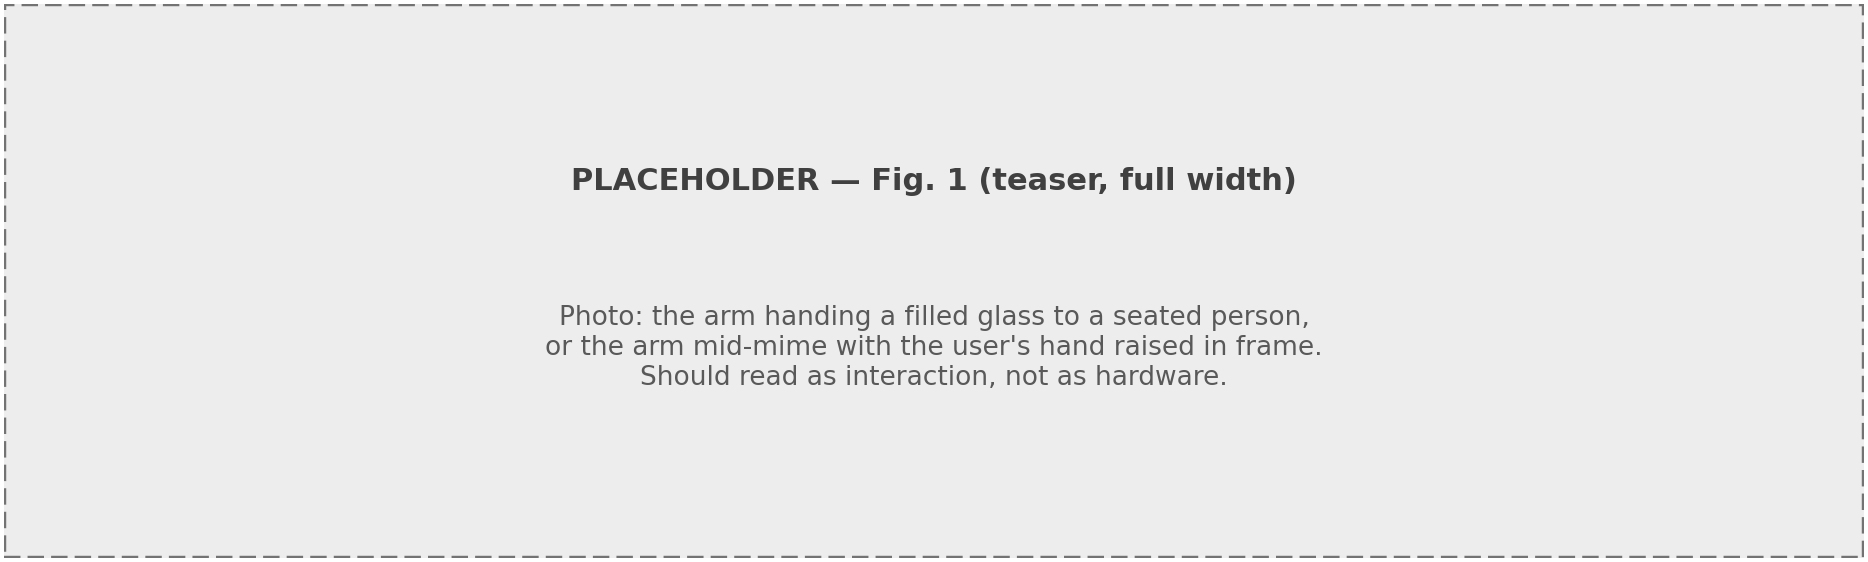
\includegraphics[width=\linewidth]{figures/teaser.png}
  \caption{BrewBot offering and serving a drink in the lab kitchen. The arm
  hangs from a ceiling rail, so it can travel between the sink, the coffee
  machine and the person it is serving.}
  \Description{A robot arm mounted on a ceiling rail hands a glass to a seated
  person in a kitchen.}
  \label{fig:teaser}
\end{teaserfigure}



\maketitle

% Use this file to enter your text.

\section{Introduction and Related Work}

A service robot is typically reactive: the human makes a request and the robot
responds. Physiological and contextual sensing enables a different form of
interaction. Rather than waiting until a person explicitly asks for assistance,
a robot can use cues about the person's current physical or affective state to
decide that assistance might be appropriate and proactively offer it. This idea
is particularly relevant to human--robot interaction (HRI), where assistance may
involve physical action in a shared environment rather than only information or 
recommendations.

Physiological signals such as heart rate and electrodermal activity (EDA) are
commonly used as indicators for autonomic arousal and stress
\cite{healey2005stress, kim2018hrv}. Wearable devices make such signals
continuously available outside tightly controlled laboratory setups, although
substantial inter-individual variation and limitations in signal quality remain
\cite{schuurmans2020e4, vanlier2020protocol}. This relates to Schmidt's concept 
of implicit interaction, in which systems respond to contextual cues that the 
user did not deliberately produce as commands \cite{schmidt2000implicit}.
Human-state-aware interaction therefore offers an opportunity for robots to
adapt without requiring the user to repeatedly articulate their needs.

Proactivity introduces an additional problem, however. A command-driven robot is
normally addressed at a time selected by the human. A proactive robot instead
chooses when to initiate an interaction. Research on proactive HRI consequently
emphasizes not only whether robots should take initiative, but also the
circumstances in which such initiative is desirable
\cite{baraglia2016initiative, broek2024proactive}. A potentially useful
suggestion can still be disruptive if the user is occupied, already interacting
with another person, unable to speak, or simply uninterested. For a state-aware
robot, estimating \emph{what} might be useful and deciding \emph{when and how}
to offer it are therefore separate questions.

This becomes especially relevant when interaction is multimodal. Speech is
convenient when the user is free to converse, but it is not always the cheapest
or most appropriate response channel. Multimodal interaction research has long
argued against treating modalities as interchangeable copies of one another and
shows that users select modalities according to task and situational constraints
\cite{oviatt1999myths}. In human-agent collaboration, related mixed-initiative
perspectives emphasize that initiative and control may shift between human and
system rather than belonging exclusively to one side \cite{cila2022designing}.
For a proactive robot, multimodality can thus serve not only recognition
robustness but also \emph{user control over the interaction itself}.

We investigate these questions through BrewBot, an integrated robotic drink
assistant. BrewBot combines physiological sensing, proactive beverage
suggestions, speech, human hand gestures, robot gestures, smart-home devices,
and physical manipulation in a shared kitchen environment. The beverage-serving
task provides a concrete setting in which inferred human state can influence
robot behavior while every suggestion still requires explicit human acceptance.
We chose drink assistance because it turns an inferred state into a concrete, 
low-stakes offer: an unsuitable suggestion can be declined, changed, or ignored 
without serious consequence.

The project makes three main contributions as a design case. First, BrewBot
integrates wearable and heart-rate sensing into an end-to-end robotic assistance
pipeline in which approximate physiological state estimates inform
context-dependent beverage suggestions. Second, users can accept, reject, or
change suggestions through speech or gestures and can explicitly replace an
ongoing verbal exchange with an embodied gesture-based interaction. Third,
BrewBot connects state inference and interaction management to real physical
actions, including drink preparation through smart-home infrastructure, delivery
to different locations, and collaborative execution of tasks that cannot be
fully automated.

BrewBot was developed by a three-person student team around an intensive
on-site practical phase, with preparatory work on sensing, arm control, and the
kitchen setup before the final integration. The prototype was refined through
repeated demonstration runs rather than through a formal study. These runs were
used to test whether the complete interaction could proceed from sensed state to
suggestion, human confirmation, and physical drink delivery, and they exposed
the interruption, modality-switching, and legibility issues discussed below.

Our goal is not to claim validated inference of psychological states or superior
user experience. No controlled user study was conducted. Instead, BrewBot is
presented as an integrated prototype from which we derive design considerations
and testable hypotheses for future state-aware HRI systems.

\section{BrewBot System and Interaction Design}

\subsection{Architecture and Human-State Inference}

BrewBot operates in an instrumented lab kitchen at LMU Munich. The robotic
platform consists of a ceiling-mounted Kinova Gen3 six-degree-of-freedom arm
with a Robotiq 2F-140 gripper. The arm is attached to a motorized linear rail
that allows it to travel between relevant areas of the kitchen, including the
workstation, sink, and networked coffee machine. The system is implemented in
ROS 2 \cite{macenski2022ros2}.

Physiological sensing is distributed across a dedicated heart-rate sensor and an
Empatica E4 wristband. The E4 provides electrodermal activity, skin temperature,
and acceleration, while the separate heart-rate sensor directly reports heart
rate in beats per minute. Cameras in the environment and on the robot support gesture
recognition. Speech input is transcribed locally, speech output is produced
on site, and a locally hosted language model supports the interpretation of
free-form replies. Home Assistant connects BrewBot to smart-home infrastructure
including the coffee machine and lights. In the implemented system, these functions 
are distributed across ROS 2 nodes for sensing, state estimation, triggering, 
interaction management, speech input and output, gesture recognition, arm control, 
and smart-home actuation. This structure matters for the interaction as well as the 
architecture: sensing, interruption, dialogue, and physical action can be adjusted 
independently. When non-essential components fail, the system can still preserve 
the user's control over whether a drink is prepared or delivered.

\begin{figure*}[t]
\centering
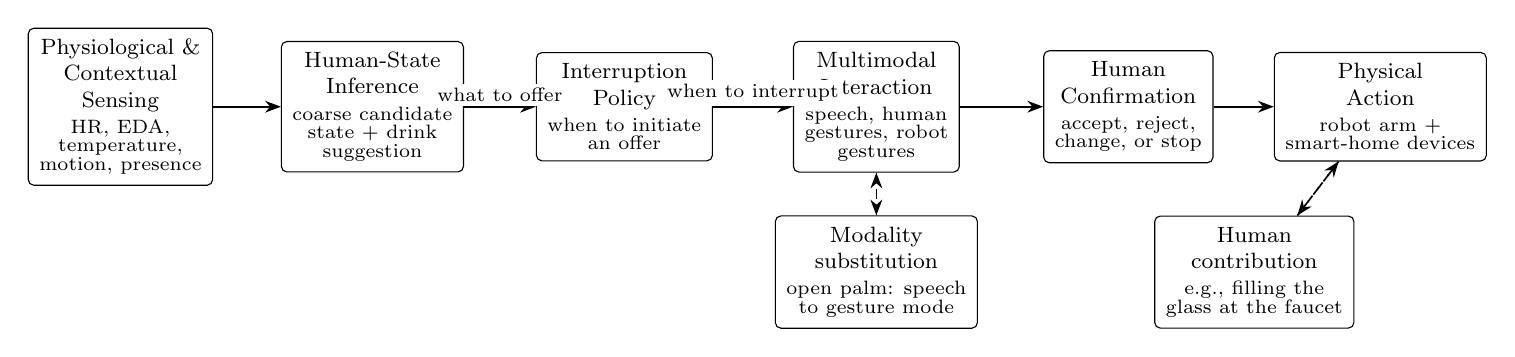
\begin{tikzpicture}[
  every node/.style={font=\small},
  box/.style={draw, rounded corners=2pt, align=center, inner sep=4pt,
              minimum height=9mm, font=\small},
  smallbox/.style={box, font=\footnotesize},
  flow/.style={-{Stealth[length=2mm]}, semithick},
  back/.style={-{Stealth[length=2mm]}, semithick, dashed},
  lbl/.style={font=\scriptsize, inner sep=1.5pt, fill=white}
]

\node[smallbox] (sense) at (0,0) {Physiological \&\\Contextual\\Sensing\\
{\scriptsize HR, EDA,}\\[-1mm]{\scriptsize temperature,}\\[-1mm]{\scriptsize motion, presence}};
\node[smallbox] (infer) at (3.2,0) {Human-State\\Inference\\
{\scriptsize coarse candidate}\\[-1mm]{\scriptsize state + drink}\\[-1mm]{\scriptsize suggestion}};
\node[smallbox] (policy) at (6.4,0) {Interruption\\Policy\\
{\scriptsize when to initiate}\\[-1mm]{\scriptsize an offer}};
\node[smallbox] (multi) at (9.6,0) {Multimodal\\Interaction\\
{\scriptsize speech, human}\\[-1mm]{\scriptsize gestures, robot}\\[-1mm]{\scriptsize gestures}};
\node[smallbox] (confirm) at (12.8,0) {Human\\Confirmation\\
{\scriptsize accept, reject,}\\[-1mm]{\scriptsize change, or stop}};
\node[smallbox] (act) at (16.0,0) {Physical\\Action\\
{\scriptsize robot arm +}\\[-1mm]{\scriptsize smart-home devices}};

\draw[flow] (sense) -- (infer);
\draw[flow] (infer) -- node[lbl, above]{what to offer} (policy);
\draw[flow] (policy) -- node[lbl, above]{when to interrupt} (multi);
\draw[flow] (multi) -- (confirm);
\draw[flow] (confirm) -- (act);

\node[smallbox] (sub) at (9.6,-2.1) {Modality\\substitution\\
{\scriptsize open palm: speech}\\[-1mm]{\scriptsize to gesture mode}};
\node[smallbox] (human) at (14.4,-2.1) {Human\\contribution\\
{\scriptsize e.g., filling the}\\[-1mm]{\scriptsize glass at the faucet}};

\draw[back] (multi) -- (sub);
\draw[back] (sub) -- (multi);
\draw[back] (act) -- (human);
\draw[back] (human) -- (act);

\end{tikzpicture}
\caption{Conceptual architecture of BrewBot. Physiological and contextual
signals are transformed into a candidate user state. The state estimator
informs, but does not itself initiate, interaction. A separate interaction
policy determines whether a suggestion should be made. Users can then respond
through speech or gestures before the accepted action is transferred to the
robot and smart-home components. Dashed feedback arrows illustrate modality
substitution and the human contribution required during collaborative tasks such
as filling a glass at the tap.}
\Description{A left-to-right conceptual diagram from physiological sensing to
human-state inference, interruption policy, multimodal interaction, human
confirmation and physical action, with feedback boxes for modality substitution
and human contribution.}
\label{fig:concept}
\end{figure*}

Conceptually, BrewBot follows a sense--infer--interact--act architecture
(\autoref{fig:concept}). A central design decision is that the state estimator
itself remains passive. It maintains the current sensor-derived state and
corresponding beverage suggestion but does not command the robot to approach or
interrupt the user. A separate trigger and interaction layer decides when a
state estimate should result in a proactive offer. This distinction separates
two questions with fundamentally different inputs:

\paragraph{What might be appropriate to offer?}
This depends primarily on physiological and activity-related cues.

\paragraph{Is it appropriate to initiate an interaction now?}
This additionally depends on interaction history, whether the user is present,
whether another interaction is already active, and whether the same state has
already triggered an offer recently.

The estimator uses a deliberately simple rule-based approach. Skin temperature,
motion, heart rate relative to a configured baseline value, and EDA relative to a
running baseline are combined into approximate user-state categories. Thermal and 
activity cues are considered before arousal-related cues so that obvious physiological
confounds, such as an elevated heart rate during movement, are less likely to be
interpreted directly as an affective state. The resulting internal states
include \emph{hot}, \emph{cold}, \emph{active},
\emph{stressed/elevated arousal}, \emph{fatigued/low arousal}, and
\emph{calm}. They map to illustrative beverage policies such as water for heat
or activity, tea for cold or elevated arousal, and coffee for low-arousal
conditions.

These labels must be understood as operational categories used by the prototype
rather than validated diagnoses. Heart rate or EDA alone do not establish that
a person is stressed, nor does reduced EDA establish fatigue. The mapping
between physiological cues, inferred state, and drink should therefore be
interpreted as a demonstrator for adaptive interaction rather than as a medical
or physiological recommendation.

Heart-rate variability (HRV) was considered during development because of its
established relation to stress \cite{kim2018hrv}. Reliably deriving
beat-to-beat intervals from the E4's wrist photoplethysmography, however,
introduced a signal-processing problem beyond the scope of the project. BrewBot
therefore uses a separate heart-rate sensor and retains the E4 primarily for
EDA, skin temperature, and motion. This pragmatic division also reflects
published validation work showing that physiological measures from wrist-worn
devices are sensitive to measurement conditions and signal quality
\cite{schuurmans2020e4, vanlier2020protocol}.

To prevent momentary fluctuations from immediately producing unsolicited
interaction, BrewBot requires persistent evidence of a relevant state change and
applies a cooldown after proactive suggestions. This is not intended to solve
the broader problem of interruption timing, but it avoids a simple failure mode
in which noisy or persistent physiological conditions cause repeated offers.

\subsection{Proactive and Multimodal Interaction}

BrewBot treats physiological inference as a basis for offering assistance, not 
as an authorization to act. Even when BrewBot derives a candidate state and 
corresponding beverage, it does not automatically prepare the drink. 
Instead, the robot makes an offer and waits for confirmation. The user may 
accept, reject, or request another available beverage. This distinction 
preserves human agency despite the proactive nature of the system.

The default interaction channel is verbal. BrewBot can address the user,
explain or contextualize its suggestion, and ask whether the proposed drink is
desired. Speech recognition converts the reply to text, after which a locally
hosted language model classifies the response into a restricted set of
meaningful outcomes. This allows responses that are more expressive than simple
yes/no answers. For example, a reply such as ``No, but I'd rather have coffee''
can be interpreted simultaneously as rejection of the suggestion and selection
of an alternative beverage.

The language model is intentionally kept outside the robot's physical control
path. It can generate or interpret language but cannot introduce unsupported
drinks or directly select robot motions. If language processing fails, BrewBot 
falls back to predefined prompts and responses. This confines the least 
deterministic component of the system to communication rather than physical 
control.

\begin{figure}[t]
\centering
\begin{subfigure}[b]{0.31\linewidth}
  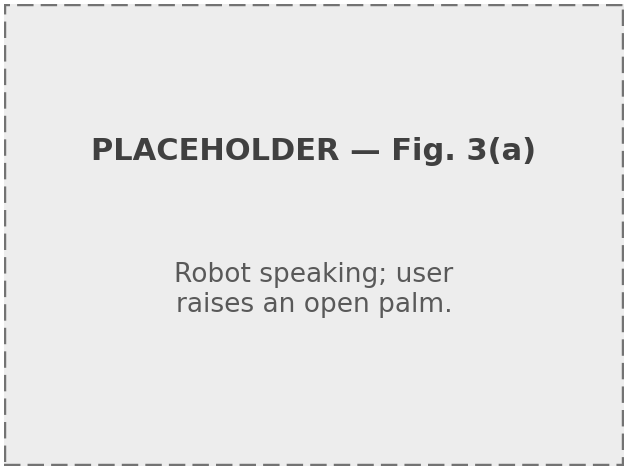
\includegraphics[width=\linewidth]{figures/palm.png}
  \caption{}\label{fig:mod-a}
\end{subfigure}\hfill
\begin{subfigure}[b]{0.31\linewidth}
  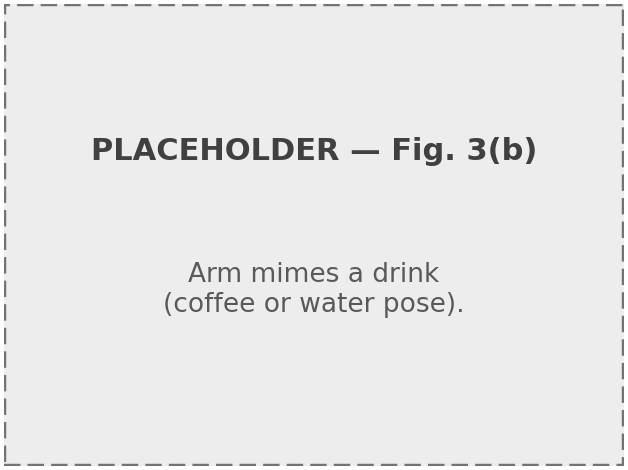
\includegraphics[width=\linewidth]{figures/mime.png}
  \caption{}\label{fig:mod-b}
\end{subfigure}\hfill
\begin{subfigure}[b]{0.31\linewidth}
  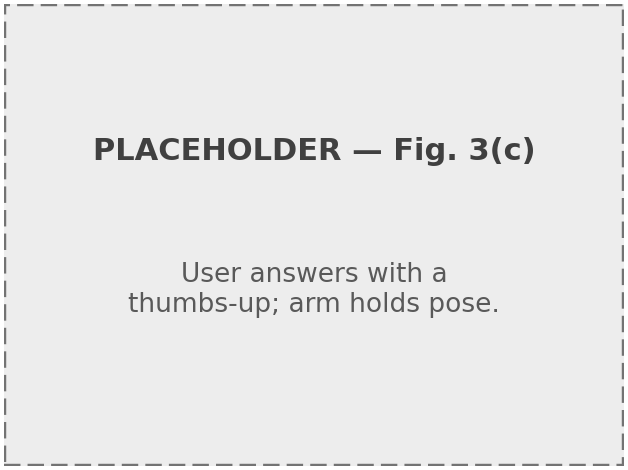
\includegraphics[width=\linewidth]{figures/thumb.png}
  \caption{}\label{fig:mod-c}
\end{subfigure}
\caption{Modality substitution in BrewBot. (a) The user raises an open palm
during a verbal offer, stopping the speech channel. (b) The robot continues the
interaction by physically miming the available beverage options. (c) The user
accepts or rejects the currently presented option with a thumbs-up or
thumbs-down. The interaction therefore continues after the user has rejected
the original communication modality.}
\Description{Three photographs showing a user raising a palm, a robot arm
performing a drink-miming motion, and the user giving a thumbs-up.}
\label{fig:modality}
\end{figure}

Human hand gestures provide a second reply channel. MediaPipe
\cite{lugaresi2019mediapipe} is used to recognize three deliberately restricted
gestures: thumbs up, thumbs down, and open palm. Recognition is stabilized
across consecutive frames before a gesture is accepted. Gesture semantics depend
on the interaction context rather than being defined globally. A thumbs-up may
indicate acceptance of a drink offer, while during another task it can indicate
that a human contribution has been completed.

The "open-palm" gesture illustrates this context-dependent design. During verbal 
interaction, an open palm immediately stops ongoing speech. It then publishes 
a stop signal for text-to-speech and marks the drink request so that the arm 
controller offers the menu through predefined mime motions. The gesture therefore 
rejects the current communication modality, but not necessarily the underlying 
offer. BrewBot can then transfer the remaining interaction from speech to an 
embodied gesture mode.

In gesture mode, the robot represents available beverages through predefined arm
and gripper motions. It orients toward a predefined user-facing pose, performs
the corresponding drink gesture, and waits for feedback. A thumbs-up selects the
presented drink; a thumbs-down proceeds to another option; an additional
open-palm response can end the offer.

This distinction leads to an important design observation: \emph{rejecting a
modality is not necessarily the same as rejecting the interaction}. BrewBot
therefore treats speech and gesture as substitutable channels rather than merely
two interfaces available in parallel. The open palm functions as a form of
modality negotiation: the human can determine not only the answer to the robot's
question, but also how the conversation should proceed.

\subsection{Embodied Drink Assistance}

Once a beverage is explicitly accepted, interaction becomes physical. BrewBot 
combines stored task poses with motion planning to pick up a glass or cup, 
travel between stations using the ceiling rail, interact with available 
appliances, and deliver the resulting drink to a predefined location such as 
the user's desk.

Coffee and hot water for tea can be requested through the networked coffee
machine via Home Assistant and Home Connect. The robot places the cup at the 
coffee machine, starts the drink program through Home Assistant, waits for 
dispensing, and then delivers the cup. The details of motion planning are 
deliberately secondary to the HRI design: from the user's perspective, the 
important property is that a conversational or gestural decision leads to a 
visible physical outcome in the shared environment.

Water requires a different interaction pattern because BrewBot cannot operate 
the tap itself. The robot picks up a glass, positions it under the faucet, and 
requests human assistance through the interaction system while holding the glass 
in place. The human opens the tap, fills the glass, and closes it again before 
signalling completion through speech or gesture. Rather than treating the 
inability to manipulate the faucet as a failure, the task becomes a small 
instance of \emph{human--robot collaborative execution} in which each participant
contributes the action they can perform more easily.

This interaction also exposed a problem of robot legibility. While waiting under
the faucet, a stationary arm can be difficult to distinguish from a robot that
has stopped functioning. BrewBot therefore uses staged non-verbal attention cues 
when the wait becomes prolonged: the arm first performs a small wrist movement 
while continuing to hold the glass, and then the smart lights blink to provide 
an additional environmental cue. These actions communicate system state without 
requiring repeated spoken interruptions.

The same principle motivates the robot's orientation during gesture
interaction. Turning toward the user and adding visible questioning movements is
not necessary merely for gesture recognition; it helps communicate that an
interaction is active and that the next action belongs to the human. BrewBot
thus uses physical motion both instrumentally, to manipulate objects, and
communicatively, to make the interaction state more legible.

\section{Design Reflections}

BrewBot was developed as an integrated course prototype rather than as a
controlled experiment. The following observations should therefore be
interpreted as design reflections and hypotheses, not validated design
principles.

\subsection{Separate State Inference from Interruption Policy}

An early architectural temptation in a state-aware robot is to let the inference
component directly trigger behavior: if the system identifies a relevant state,
it immediately sends a corresponding robot command. BrewBot instead separates
state estimation from interaction initiation.

This separation matters because \emph{what to offer} and \emph{when to
interrupt} depend on different information. Physiological measurements may
suggest that water or another beverage could be appropriate, but they do not
indicate whether the user is currently available for interaction. Arrival,
recent offers, an ongoing dialogue, previous rejection, and the persistence of a
sensor condition all influence whether initiating another interaction is
sensible.

Keeping these responsibilities separate also makes different intervention
policies possible without changing the state estimator. More sophisticated
future policies could incorporate explicit availability cues, task context,
learned interruption preferences, or confidence in the estimated state while
retaining the same sensing pipeline.

\subsection{Make Modalities Substitutable and Preserve User Agency}

Simply supporting speech and gestures does not make an interaction meaningfully
multimodal. BrewBot's more consequential design choice is that one channel can
replace another while preserving the interaction state.

The open-palm mechanism illustrates this directly. The user can reject speech
without rejecting the underlying beverage offer, after which the robot continues
through physical gestures. Gesture meanings are furthermore interpreted relative
to the current question, allowing the same limited vocabulary to function under
different physical constraints.

This design is closely connected to human agency. BrewBot initiates interaction
based on information the user did not deliberately provide as a command. Such
implicit input should not silently become authorization for physical action. We
therefore maintain the sequence:
\begin{quote}
sensed cue $\rightarrow$ candidate state $\rightarrow$ suggestion $\rightarrow$
human confirmation $\rightarrow$ physical action
\end{quote}
rather than:
\begin{quote}
sensed cue $\rightarrow$ inferred state $\rightarrow$ physical action
\end{quote}

The human can accept the suggestion, reject it, choose an alternative, change
the communication modality, or terminate the interaction. In this sense,
proactivity determines who may \emph{start} the interaction, but not who has
final authority over the resulting action.

\section{Limitations}

BrewBot was demonstrated and iteratively developed by the project team, but 
the system was not evaluated with independent participants in a user study. 
We therefore cannot conclude that its proactive behavior is perceived as 
useful rather than intrusive, that its robot gestures are intuitively 
understandable, or that allowing users to (seamlessly) switch modalities 
improves the interaction.

A second limitation concerns human-state inference. The current estimator is
heuristic and has not been calibrated against self-reported ground truth.
Physiological measures vary substantially between people and can be affected by
movement, environment, sensor placement, and other factors unrelated to the
states represented by BrewBot's labels. Although relative baselines and explicit
handling of some physical confounds improve the rule set, the resulting
categories remain tentative hypotheses rather than validated state estimates.

The mapping from states to beverages is similarly illustrative. A person with
elevated arousal does not necessarily want tea, and a low-arousal signal does
not imply that coffee is desirable. Beverage selection is therefore best
understood as an adaptive interaction policy chosen for the prototype. A
deployable system would need a preference model or recommender component that 
learn from repeated acceptance and rejection rather than apply one mapping to 
all users.

The physical system also relies strongly on a structured environment. Many
poses and object locations are predefined, which limits robustness when cups or
other objects are moved. The current interaction was tested over
demonstration-length sessions rather than long-term deployment, so the
acceptability of proactive offers over several hours or days remains untested.

Finally, physiological sensing raises privacy considerations beyond those of a
conventional drink-serving robot. Signals such as heart rate and EDA constitute
personal data and may permit inferences users did not explicitly intend to
communicate. The prototype operates locally in a research environment, but
long-term use would require explicit decisions about consent, transparency,
storage, retention, and the user's ability to disable state-aware behavior.

\section{Future Work}

An empirical evaluation of the interaction design would be a useful next step, 
alongside further robotic capabilities. A within-subjects study could compare 
proactive state-aware assistance with user-initiated service, measuring 
perceived intrusiveness, usefulness, trust, usability, and task load. 
A second factor could compare speech-only interaction with the substitutable 
speech-and-gesture design. Such a study would directly test the hypothesis 
emerging from BrewBot that allowing users to replace an inconvenient interaction 
modality can make proactive assistance easier to manage.

Gesture comprehensibility is another open question. The human gestures used by
BrewBot are intentionally simple, but the robot's beverage mimes are designed
rather than universally established symbols. Future work should therefore test
whether users can correctly interpret these gestures without prior instruction
and whether different robot motions convey waiting, questioning, or offering
states as intended.

Human-state inference should also become individualized and uncertainty-aware. A
short calibration phase could establish personal baselines for physiological
measures, while repeated interaction could allow the system to learn individual
mappings between state, context, and beverage preference. Instead of treating a
rule as ``low arousal implies coffee,'' the system could learn that a particular
user repeatedly chooses water or declines assistance in that context. Confidence
estimates could additionally allow BrewBot to refrain from proactive interaction
when the available sensor evidence is ambiguous.

Longer-term interaction also requires adaptive interruption policy. Repeated
rejection should influence future behavior, and the system should learn both
\emph{what} a person tends to accept and \emph{when} they prefer not to be
interrupted. This would extend BrewBot from a state-aware system toward a
genuinely personalized mixed-initiative assistant.

On the physical side, fiducial markers such as AprilTags
\cite{olson2011apriltag} or more general object perception could reduce
dependence on hard-coded poses and enable dynamic cup pickup and placement.
Detecting whether a cup is present or empty could also provide task-context
information that complements physiological sensing. Such environmental evidence
may in many situations be more directly relevant to the need for a refill than a
physiological cue alone.

\section{Conclusion}

BrewBot demonstrates an end-to-end approach to human-state-aware robotic
assistance in which physiological sensing, proactive interaction, multimodal
communication, smart-home integration, and embodied action are connected within
one system. The central challenge that emerged was not simply how to infer a
state or how to deliver a drink, but how a robot should negotiate assistance
when it initiates the interaction itself.

Three design considerations summarize this experience. First, estimating
\emph{what} might be useful should be separated from deciding \emph{when}
interaction is appropriate. Second, multimodal interaction becomes more
meaningful when modalities can substitute for one another according to the
user's situation. Third, state inference should inform a proposal rather than
remove human authority over the resulting action.

BrewBot therefore treats physiological state not as an instruction, but as a
reason to ask. The robot may take the initiative, but the user decides whether
the interaction continues, which modality it uses, and what the robot ultimately
does.


%TC:ignore
\bibliographystyle{ACM-Reference-Format}
\bibliography{bibliography}

\appendix
\section*{Character Count}
This work contains \charactercount{content} characters (without spaces).
%TC:endignore
\end{document}
